%%%%%%%%%%%%%%%%%%%%%%%%%%%%%%%%%%%%%%%%%%%%%%%%%%%%%%%%%%%%%%%%%%%%%%%%%%%%%%%%
%%%% オペレーションズ・リサーチ　各種記事ひな形LaTeX2eファイル　2015-08-31版 %%%
%%%%%%%%%%%%%%%%%%%%%%%%%%%%%%%%%%%%%%%%%%%%%%%%%%%%%%%%%%%%%%%%%%%%%%%%%%%%%%%%
\documentclass[twocolumn, lastpage]{jarticle}

% nidanfloat（2段抜きフロートの[tb]配置）と新しいLaTeXのmarks機構の非互換による
% 「! LaTeX mark Error: Infinite shrinkage found in 'column'.」を抑制する。
% このテンプレートのヘッダは固定文字列でmarksを使わないため、組版への実害はない。
\ExplSyntaxOn
\msg_redirect_name:nnn { mark } { infinite-shrinkage } { none }
\ExplSyntaxOff

\overfullrule=5pt

\usepackage{amsmath,amssymb,amsfonts}
\usepackage{bm}
\usepackage{placeins}
\usepackage{graphicx}
\usepackage{subcaption}
\renewcommand{\thesubfigure}{(\alph{subfigure})}
\captionsetup[subfigure]{labelformat=simple}
\usepackage{nidanfloat}
\usepackage[numbers,sort]{natbib}
\usepackage{color}
\usepackage{url}
\usepackage{comment}

%%%%%%%%%%%%%%%%%%%%%%%%%%%%%%%%%%%%%%%%%%%%%%%%%%%%%%%%%%%%%%%%%%%%%%%%%%%%%%%%
%%% 査読対応の修正箇所マーク
%%%
%%% 【見た目（PDF）で分かる方法】
%%%   \revA{...} … 査読者#A への対応（青色）
%%%   \revB{...} … 査読者#B への対応（赤色）
%%%   別行立ての数式や図表などブロック要素には
%%%   \revAblock{...} / \revBblock{...} を用いる．
%%%   最終稿では下の \revmarktrue を \revmarkfalse に変えるとマークが消える．
%%%   （日本語＋段組では ulem/soul の下線が折り返せないため，色のみで示している）
%%%
%%% 【TeXソース上で分かる方法】
%%%   各修正は  %%% [REV-A1] ... ここから  〜  %%% [REV-A1] ここまで  で囲む．
%%%   A1/A2... は査読者#Aのコメント番号，B1/B2... は査読者#Bのコメント番号に対応．
%%%   grep -n "REV-A" main.tex  で修正箇所を一覧できる．
%%%%%%%%%%%%%%%%%%%%%%%%%%%%%%%%%%%%%%%%%%%%%%%%%%%%%%%%%%%%%%%%%%%%%%%%%%%%%%%%
\usepackage{multirow}
\newif\ifrevmark
\revmarktrue   % 最終稿では \revmarkfalse に変更する
\newcommand{\revA}[1]{\ifrevmark{\color{blue}#1}\else#1\fi}
\newcommand{\revB}[1]{\ifrevmark{\color{red}#1}\else#1\fi}
\newcommand{\revAblock}[1]{\ifrevmark{\color{blue}#1}\else#1\fi}
%%%   図表（float）の中は外側の色が届かないため，\begin{table}直後に \revAcolor を置く．
\newcommand{\revAcolor}{\ifrevmark\color{blue}\fi}
\newcommand{\revBcolor}{\ifrevmark\color{red}\fi}
\newcommand{\revBblock}[1]{\ifrevmark{\color{red}#1}\else#1\fi}

\usepackage{or}
\AtBeginDvi{\special{papersize=210mm,297mm}}

\vol{}
\vnum{}
\vyear{2026}

\jtitle{Gate Retrieval-Augmented Forecastingによる\\書籍需要予測}
% \jauthor{奈良原 俊誠，斎藤 陽，橋本 朋樹，三川 健太}
\jauthor{}
% \autfuri{ならはら　しゅんせい，さいとう　はる，はしもと　ともき，みかわ　けんた}
\autfuri{}
\shozoku{}
%\shozoku{東京都市大学メディア情報学部情報システム学科}
%\shozoku{〒224--0015\enspace 神奈川県横浜市都筑区牛久保西3-3-1}

\begin{comment}
% 複数のメールアドレスは，見栄えに応じて改行を挿入すること
\shozoku{or-taro@sankaku.maru.ac.jp,\\ or-hanako@sankaku.maru.ac.jp}
% 住所のみ記載の例
\autfuri{おーあーる　じろう}
\shozoku{□□（株）☆☆☆☆部}
\shozoku{〒000--0000\enspace ■■県★★市◆◆区▼▼▼▼0--0--0}
% メールアドレスのみ記載の例
\autfuri{おーあーる　さぶろう}
\shozoku{◇◇大学▽▽学部}
\shozoku{or-saburo@shitasankaku.hishi.ac.jp}
% 外国所属で，住所のみ記載の例
\autfuri{ヤン　ヤンセン}
\shozoku{Department of AAA, BBB University of Technology}
\shozoku{P.O. Box 1111, 2222 GA Delft, The Netherlands}
% “論文・事例研究”・“論文・研究レポート”の場合，
% この位置に論文受付・採録に関係する日付が記載される
%\shozoku{受付 15.8.15　採択 15.8.15}
% “学生論文賞受賞論文”の場合↓
%\shozoku{
%○○大学大学院△△研究科 \\
%（現所属：□□（株）☆☆☆☆部） \\
%指導教員：尾有太郎　教授
%}
% “特集にあたって”の場合は，なし
\end{comment}


\begin{comment}
%% あらまし
% “特集記事”の場合に限り，必ず使用すること↓
\jabstract{
これは，オペレーションズ・リサーチ誌の各種記事の
ひな形（2015年8月31日版）である．
“特集記事”・“論文・事例研究”・“論文・研究レポート”
・“ORメモランダム”の場合に限り，サブタイトルを記載してもよい．
“特集記事”の場合に限り，あらましをここに，280字以内で記載し，
その下にキーワードを記載する．
}

\jkeywords{
特集記事キーワード1，キーワード2，
キーワードは三つ以上（指定のキーワードは特になし）
}
\end{comment}


\begin{document}
\special{papersize=210mm,297mm}
\normalsize
\setcounter{page}{1}
\setcounter{secondpage}{1}
\maketitle


%%%%%%%%%%%%%%%%%%%%%%%%%%%%%%%%%%%%%%%%%%%%%%%%%%%%%%%%%%%%%%%%%%%%%%%%%%%%%%%
\section{はじめに}
%%%%%%%%%%%%%%%%%%%%%%%%%%%%%%%%%%%%%%%%%%%%%%%%%%%%%%%%%%%%%%%%%%%%%%%%%%%%%%%
出版物は，個々の販売規模が小さく品目数が多いという多品種少量生産の性質をもつ．こうした多様な出版物の流通を支えるため，出版業界では再販売価格維持制度と委託販売制度が広く用いられている．前者は出版社が定価を定めて小売店に定価での販売を求める制度であり，価格競争による淘汰から多様な出版物を守る~\cite{JBPA.2001}．後者は，小売店が売れ残った在庫を出版社へ返品できる委託仕入れの制度であり，小売店の在庫リスクを抑える一方で，返本を構造的に生み出す．
需要に基づかない発注や配本は，この返本をさらに増大させる．返本の増加は物流コストや流通効率の面で出版業界全体の課題となっており~\cite{Shuppan.2024}，返本率の低減には需要に即した配本が不可欠である．したがって，書籍の販売冊数を適切に予測することは，出版流通の効率化における重要な課題である．

一般に，書籍の需要予測は，過去の販売冊数に基づく時系列予測問題として位置づけられる．しかし多品種少量生産という特性上，需要の多くはゼロや少数にとどまる一方で，初版発行やイベントなどにより突発的な需要増加が生じる．通常の予測モデルはこうした需要を平坦に予測しやすく，単一系列の履歴だけでは稀にしか起こらないスパイクのパターンを学習しにくい．

時系列予測問題に対し，自然言語処理のRetrieval-Augmented Generation（RAG）~\cite{Lewis.2020}を時系列予測へ拡張したRetrieval-Augmented Forecasting（以下，RAF）が提案されている~\cite{Tire.2024}．RAFは，予測対象の直近の変動パターンに類似する過去の部分系列（以下，参照ウィンドウ）をデータベースから検索し，予測モデルへの追加情報として利用する．これにより類似事例を系列横断的に活用できるため，予測対象系列のみを用いる単一系列モデルでは捉えにくい情報を補うことができる．
しかしながら従来のRAFは，参照ウィンドウを予測対象の直近区間に時間軸方向へ連結して入力するため，主に二つの問題を抱える．
第一に，参照ウィンドウと直近区間では値の水準や端部の変化が必ずしも一致せず，両者の接続点に不連続が生じる可能性がある．
第二に，近傍探索は相対的な類似順位で検索結果を選ぶため，予測に十分関連しない参照ウィンドウであっても一律に取り込まれてしまう．

上記の議論を鑑み，本研究では従来のRAFの持つ問題を解決し，
書籍の販売冊数を高精度に予測する手法の構築を目的とする．
このために，上記の問題に対処したゲート付き融合型RAFであるGateRAFを提案する．
GateRAFでは，ローカルコンテキストと各参照ウィンドウを同一のエンコーダで独立に処理するマルチストリームエンコードを導入し，入力系列の接合に伴う不連続性を排除する．さらに，ローカル要約ベクトルと各参照パッチとの関連度をスカラーゲートによって評価することで，予測対象との関連性が低い参照情報の混入を動的に抑制する．

提案手法の有効性を，経営科学系研究部会連合協議会が主催する令和7年度データ解析コンペティションより提供された書籍POSデータを用いた実験により検証する．
実験を通じて，GateRAFが従来手法に対して予測精度を改善すること，平常時の過大予測の抑制とスパイク近傍の予測の時間的な改善にそれぞれ寄与することを示す．



%%%%%%%%%%%%%%%%%%%%%%%%%%%%%%%%%%%%%%%%%%%%%%%%%%%%%%%%%%%%%%%%%%%%%%%%%%%%%%%
\section{準備}
%%%%%%%%%%%%%%%%%%%%%%%%%%%%%%%%%%%%%%%%%%%%%%%%%%%%%%%%%%%%%%%%%%%%%%%%%%%%%%%
\subsection{問題設定}
本研究では，経営科学系研究部会連合協議会が主催する令和7年度データ解析コンペティションより提供いただいた書籍POSデータを使用する．本データは2024年の1年間にわたる全国35店舗分の書籍・雑誌の販売実績であり，約20万書名・約400万件の販売記録から構成される．各記録は販売日，店舗，書名，販売冊数等の情報を持つ．

前述の通り，書籍の販売冊数は，平常時には少数にとどまることが多い一方，イベントなどに起因して短期間だけ販売冊数が急増する場合がある．以下では，このような一時的な需要増加をスパイクと呼ぶ．
需要を過小に見積もればスパイクが発生した際に機会損失が生じ，逆に過大に見積もれば在庫や返本の増加につながる．
したがって本研究では，平常時の少数需要とスパイクが混在する販売冊数を，過不足なく予測することを課題とする．
%%% [REV-A5] 目的変数の明記（査読者#A コメント5）ここから
\revA{予測の対象は，書名ごとに全店舗の販売冊数を日単位で合算した時系列であり，目的変数は将来の各日における販売冊数そのものである．すなわち，一定期間の累計販売冊数ではなく，1日単位の販売冊数を予測の対象とする．}
%%% [REV-A5] ここまで
%%% [REV-A6] 「需要」と販売冊数の関係の定義（査読者#A コメント6）ここから
\revA{本研究で観測できるのは実際に販売された冊数であり，これを販売冊数と呼ぶ．消費者が買いたいと考えた量である需要は，在庫切れがあれば販売冊数を上回るが，本研究のPOSデータには在庫情報がないため観測できない．そこで販売冊数を需要の代理指標とし，需要予測は販売冊数の予測を指すものとする．}
%%% [REV-A6] ここまで
その際，書籍の販売特性を踏まえ，需要を平均的に均して予測するのではなく，平常時とスパイクが混在する需要構造に対応できる予測を目指す．

\subsection{関連研究}

スパイク需要の捕捉と少数系列からの学習に関連する手法は，主に時系列予測の基盤手法，間欠・突発需要予測，検索拡張型予測に分けられる．

時系列予測の基盤手法としては，PatchTST~\cite{Nie.2023}などのTransformerベースの深層学習手法，確率的予測手法であるDeepAR~\cite{Salinas.2020}やTFT~\cite{Lim.2021}，大規模事前学習基盤モデルであるChronos~\cite{Ansari.2024}が代表的な手法として挙げられる．
また，間欠・突発需要予測についても数多くの研究が存在し，Croston法~\cite{Croston.1972}が基準手法として広く参照されている．

RAG~\cite{Lewis.2020}を時系列予測へ拡張したRAFは，予測対象のローカルコンテキストに類似した過去のウィンドウを検索データベースから取得し，予測に活用する手法である．
これにより，単一系列からは捕捉が困難な稀なスパイクパターンを，系列横断的に参照できる．
代表的な手法として，Chronos~\cite{Ansari.2024}を基盤とし，検索した参照ウィンドウをローカルコンテキストへ時間軸方向に連結して，一つの拡張シーケンスとしてエンコードするProtoRAF~\cite{Tire.2024}がある．
また，TS-RAG~\cite{Ning.2025}やTimeRAF~\cite{Zhang.2024}では，それぞれ潜在空間での融合やChannel Promptingによって，検索情報の活用方法を改善している．
%%% [REV-A1] 類似尺度の選択に関する関連研究の追加（査読者#A コメント1）ここから
\revA{また，Cross-RAG~\cite{Lee.2026}は，検索された参照ウィンドウの有用性が一様ではない点に着目し，予測対象との関連度に応じて参照をクロスアテンションで重み付けする枠組みを提案している．}
%%% [REV-A1] ここまで


\section{従来手法}
提案手法の基礎となるProtoRAF~\cite{Tire.2024}は，参照ウィンドウを以下の手順で取得する．
まず，学習データの系列を長さ$L$のウィンドウに区切り，各ウィンドウを$\bm{w}_i \in \mathbb{R}^{L}$として過去のウィンドウ集合$\mathcal{D} = \{\bm{w}_i\}_{i=1}^{N}$を構成する．ただし，$N$をウィンドウ数とする．また，予測対象の直近$L$時点をローカルコンテキスト$\bm{x} \in \mathbb{R}^{L}$とおく．
ProtoRAFによる予測では，$\bm{x}$と$\mathcal{D}$の各ウィンドウ$\bm{w}_i$を互いに標準化したもとで比較する．
すなわち，$\bm{x}$を標準化した$\tilde{\bm{x}}$と，$\bm{w}_i$を標準化した$\tilde{\bm{w}}_i$の距離$d(\tilde{\bm{x}},\, \tilde{\bm{w}}_i)$を算出し，このうち距離の小さい上位$K$件を参照ウィンドウ$\bm{r}_k \in \mathbb{R}^{L}$（$k = 1, \dots, K$）として取得する：
    \begin{equation}
        \{\bm{r}_k\}_{k=1}^{K}
        = \operatorname*{Top\text{-}K_{\mathrm{min}}}_{\bm{w}_i \in \mathcal{D}}\;
        d(\tilde{\bm{x}},\, \tilde{\bm{w}}_i)
    \end{equation}
ここで，$\operatorname{Top\text{-}K_{\mathrm{min}}}$は距離$d$が小さい順に上位$K$件を選ぶ操作であり，その計算には近傍検索を用いる．
%%% [REV-A1] 距離関数dの明記（査読者#A コメント1）ここから
\revAblock{なお本研究では，距離$d$として，標準化後のウィンドウ間の二乗ユークリッド距離
    \begin{equation}\label{eq:distance}
        d(\tilde{\bm{x}},\, \tilde{\bm{w}}_i)
        = \sum_{t=1}^{L} \left( \tilde{x}_t - \tilde{w}_{i,t} \right)^{2}
    \end{equation}
を用いる．ここで$\tilde{x}_t$と$\tilde{w}_{i,t}$は，それぞれ$\tilde{\bm{x}}$と$\tilde{\bm{w}}_i$の第$t$要素を表す．この距離は標準化後の系列に対して定義されるため，系列の水準や振幅の違いを除いた変動の形状の類似度を測ることになる．}
%%% [REV-A1] ここまで

%%% [REV-A1] 距離関数dの選択が結果に与える影響（査読者#A コメント1）ここから
\revA{距離$d$の選択は，取得される参照ウィンドウそのものを変えるため，予測結果に影響し得る．たとえば標準化を行わない距離を用いれば系列の水準や振幅の近さが反映され，動的時間伸縮法を用いれば時間軸のずれを許容した照合が行われるため，いずれも式~\eqref{eq:distance}とは異なる参照ウィンドウが取得される．一方で，参照を関連度に応じて重み付けして統合する枠組みでは，類似尺度を変えても予測精度がほとんど変化しないことが報告されている~\cite{Lee.2026}．提案手法のゲート機構も参照の関連度に応じた重み付けを行い，予測対象との関連が薄い参照の寄与を抑制する．したがって，距離$d$の選択により取得される参照ウィンドウが変化しても，予測結果への影響は限定的であると考えられる．ただし本研究では距離を式~\eqref{eq:distance}に固定しており，複数の尺度を比較した検証は今後の課題である．}
%%% [REV-A1] ここまで
また，データリークを防ぐためウィンドウ集合$\mathcal{D}$は予測時点より前のウィンドウのみで構成する．この検索は$\mathcal{D}$の中で相対的に類似した上位$K$件を返すため，予測対象に真に似た事例があるか否かによらず，常に$K$件が選出される．

図~\ref{fig:protoraf}に示すように，ProtoRAFはローカルコンテキスト$\bm{x}$の前方に参照ウィンドウ$\bm{r}_1, \dots, \bm{r}_K$をそのまま連結して拡張コンテキスト$\bm{x}^{\mathrm{proto}}\in \mathbb{R}^{(K+1)L} $を構成し，これを単一シーケンスとしてエンコーダに入力してパッチ表現$H^{\mathrm{proto}}\in \mathbb{R}^{(K+1)P \times D}$を得る．パッチ数を$P$，エンコーダの埋め込み次元を$D$とすると，これらは以下のように表される：
    \begin{align}
        \bm{x}^{\mathrm{proto}} &= \mathrm{Concat}(\bm{r}_1,\, \bm{r}_2,\, \dots,\, \bm{r}_K,\, \bm{x})\\
        H^{\mathrm{proto}} &= \mathrm{Encode}(\bm{x}^{\mathrm{proto}})
    \end{align}
ここで$\mathrm{Concat}(\cdot)$は，与えられたベクトルまたは行列を行方向（時間軸方向）に連結する操作を表す．また$H^{\mathrm{proto}}$は，$\bm{x}^{\mathrm{proto}}$をパッチごとに区切って各パッチを$D$次元ベクトルへ変換し，これら$(K+1)P$個のベクトルを行方向に積み上げた$(K+1)P \times D$の行列である．
このエンコーダ$\mathrm{Encode}(\cdot)$は，入力系列をその平均と標準偏差で標準化してからパッチ表現へ変換する~\cite{Kim.2022}．
ProtoRAFでは，この標準化に用いる平均と標準偏差を，ローカルコンテキストだけでなく参照ウィンドウまで連結した$\bm{x}^{\mathrm{proto}}$全体から計算する．
    \begin{figure*}[t]
        \centering
        
\includegraphics[width=0.75\linewidth]{figure/architecture/architecture_ProtoRAF.eps}
        \caption{ProtoRAFのアーキテクチャ概要}
        \label{fig:protoraf}
    \end{figure*}

ProtoRAFは，参照ウィンドウとローカルコンテキストを1本の系列として連結する構造に起因して，接合部の不連続性と無関係な参照ウィンドウの混入という2つの問題を持つ．
前者について，$\bm{x}^{\mathrm{proto}}$では性質の異なる参照ウィンドウとローカルコンテキストが結合されるため，その境界で値の水準や形状が大きく異なりうる．エンコーダはこの不自然な結合を，データに実際に起きた変化と区別できないまま学習し，予測精度を低下させる．
加えて，この連結は標準化の基準にも影響を及ぼす．エンコーダは平均と標準偏差を$\bm{x}^{\mathrm{proto}}$全体から計算するため，大きく外れた観測値を含む参照ウィンドウが混在すると，ローカルコンテキストが本来とは異なるスケールで標準化される．
後者について，前述の通りProtoRAFは，予測対象に似た事例があるか否かによらず常に上位$K$件を返す．そのため，似た事例が乏しい場合には，関連の薄いウィンドウまで参照として連結される．ProtoRAFはこれらをローカルコンテキストと区別せず一括で符号化するため，無関係な情報も予測に取り込まれ，精度が低下する可能性が存在する．



%%%%%%%%%%%%%%%%%%%%%%%%%%%%%%%%%%%%%%%%%%%%%%%%%%%%%%%%%%%%%%%%%%%%%%%%%%%%%%%
\section{提案手法}
%%%%%%%%%%%%%%%%%%%%%%%%%%%%%%%%%%%%%%%%%%%%%%%%%%%%%%%%%%%%%%%%%%%%%%%%%%%%%%%
\subsection{概要}
前述の通り，ProtoRAFには接合部の不連続性と無関係な参照ウィンドウの混入という問題が存在する．
提案手法では，ProtoRAFの2つの問題がいずれも参照ウィンドウとローカルコンテキストを単一の系列として一括で符号化することに起因する点に着目し，
これらをそれぞれ独立に符号化し，予測に役立つ参照だけを選んで組み合わせることで改善を図る．
具体的には，マルチストリームエンコードとゲート機構の2つをProtoRAFに導入する．
マルチストリームエンコードは，ローカルコンテキストと各参照ウィンドウを個別に標準化し，共通のエンコーダで独立に符号化を行う．
これにより，系列の連結境界をデータの変化と取り違える問題と，スケール差の影響を抑える．
ゲート機構は，ローカルコンテキストとの関連性に応じて各参照への寄与を調整し，関連性の低い参照が予測に与える影響を抑制する．
以下では提案手法をGateRAFと呼ぶこととし，その概要を図~\ref{fig:gateraf}に示す．

    \begin{figure*}[t]
        \centering
        %%% [REV-A9] 図2を拡大（査読者#A コメント9）
        
\includegraphics[width=\linewidth]{figure/architecture/architecture_GateRAF.eps}
        \caption{GateRAF（提案手法）のアーキテクチャ概要}
        \label{fig:gateraf}
    \end{figure*}

\subsection{マルチストリームエンコードとゲート機構}
GateRAFは次の5つのステップから構成される．
    \begin{description}
        \item[Step 1）] ローカルコンテキストのエンコード
        \item[Step 2）] 参照ウィンドウの独立エンコード
        \item[Step 3）] ローカル要約ベクトルの計算
        \item[Step 4）] ゲートの計算
        \item[Step 5）] ゲート付き融合
    \end{description}

Step 1ではローカルコンテキストだけを符号化し，参照ウィンドウに影響されない標準化の基準を確保する．
まず，予測対象のローカルコンテキスト$\bm{x}$だけをエンコーダに入力し，そのパッチ表現$H^{\mathrm{loc}} \in \mathbb{R}^{P \times D}$を式~\eqref{eq:loc-encode}より得る：
        \begin{equation}\label{eq:loc-encode}
            H^{\mathrm{loc}} = \mathrm{Encode}(\bm{x})
        \end{equation}
ここではローカルコンテキスト$\bm{x}$のみを入力し，その平均と標準偏差で標準化するため，参照ウィンドウに含まれるスパイクの影響を受けない．

Step 2では各参照ウィンドウを独立に符号化し，連結による接合部の作成を回避する．
すなわち，各参照ウィンドウ$\bm{r}_k$をローカルコンテキストと同じエンコーダで個別に符号化し，参照ブロック$H^{\mathrm{ret}}_k \in \mathbb{R}^{P \times D}$を得る：
    \begin{equation}\label{eq:ret-encode}
        H^{\mathrm{ret}}_k = \mathrm{Encode}(\bm{r}_k)
    \end{equation}
これにより連結部分が生じず，接合部の不連続性も避けられる．この段階では各参照を独立なブロック$H^{\mathrm{ret}}_k$として保持し，ローカルコンテキストとも他の参照とも結合しない．

Step 3ではローカルコンテキストの表現を1本のベクトルにまとめ，参照の基準とする．
$H^{\mathrm{loc}}$をパッチ方向に平均プーリングし，ローカル要約ベクトル$\bar{\bm{h}}^{\mathrm{loc}} \in \mathbb{R}^{D}$を次の通り得る：
    \begin{equation}
        \bar{\bm{h}}^{\mathrm{loc}} = \mathrm{Pool}(H^{\mathrm{loc}})
    \end{equation}
ここで$\mathrm{Pool}(\cdot)$はパッチ方向の平均プーリングを表す．

Step 4では各参照パッチを予測にどれだけ反映させるかを，ローカルコンテキストとの関連の強さに応じて決める．
具体的には，Step 3で得たローカル要約ベクトル$\bar{\bm{h}}^{\mathrm{loc}}$と，各参照ブロックの第$p$パッチ$\bm{h}^{\mathrm{ret}}_{k,p} \in \mathbb{R}^{D}$を多層パーセプトロン$\mathrm{GateMLP}$に入力し，両者の関連の強さを$0$から$1$の値$g_{k,p}$として出力する：
    \begin{equation}
        g_{k,p} = \mathrm{GateMLP}(\bar{\bm{h}}^{\mathrm{loc}},\, \bm{h}^{\mathrm{ret}}_{k,p})
    \end{equation}
$g_{k,p}$は参照パッチの重みであり，$1$に近いほどその参照を予測に強く反映し，$0$に近いほど影響を抑える．関連の薄い参照を自動的に弱めることで，無関係なウィンドウの混入を防ぐことを意図する．
また，無関係な参照に影響を受けないよう，ゲートは学習の初期にはほぼ閉じた状態，すなわち出力が$0$に近い状態から始まるよう初期化する．これにより，モデルはまず信頼できるローカルコンテキストに基づいて予測を学習し，役立つ参照だけを学習の進行とともに取り込む．

Step 5ではゲートで重み付けした参照表現をローカルコンテキストの表現と統合し，予測に用いる．
まず，各参照ブロック$H^{\mathrm{ret}}_k$の各パッチに，対応する重み$g_{k,p}$を掛け，重み付き参照ブロック$\tilde{H}^{\mathrm{ret}}_k \in \mathbb{R}^{P \times D}$を得る．次に，ローカル表現と重み付けした全参照ブロックを結合して融合表現$H^{\mathrm{gate}} \in \mathbb{R}^{(1+K)P \times D}$とする：
  \begin{align}
        \tilde{H}^{\mathrm{ret}}_k &= \bm{g}_k \odot H^{\mathrm{ret}}_k \\
        H^{\mathrm{gate}} &= \mathrm{Concat}(H^{\mathrm{loc}},\,
        \tilde{H}^{\mathrm{ret}}_1,\, \cdots,\,
        \tilde{H}^{\mathrm{ret}}_K)
  \end{align}
ここで$\bm{g}_k = (g_{k,1}, \ldots, g_{k,P})^\top$は参照ブロック$k$の各パッチのゲート値を並べたベクトルであり，$\odot$は各パッチ$p$の表現全体に同じ重み$g_{k,p}$を掛ける演算を表す．関連の薄い参照ほど重みが小さくなるため，無関係なウィンドウの混入が抑えられる．参照表現とローカル表現を結合するのはStep 5のみであり，それまでは互いに干渉しない．


\subsection{予測}
最後に，融合表現$H^{\mathrm{gate}}$から将来の販売冊数を予測する．$H^{\mathrm{gate}}$には，ローカルコンテキストとゲートで重み付けした参照の情報がまとめられている．これをデコーダに渡して各分位点の予測を出力し，符号化の際に施した標準化を元に戻す．分位点の集合を$Q$，予測する日数を$F$，標準化したスケールを元に戻す操作を$\mathrm{RevNorm}$とすると，予測値$\hat{Y} \in \mathbb{R}^{|Q| \times F}$は以下のように表される：
    \begin{equation}
        \hat{Y} = \mathrm{RevNorm}(\mathrm{Decode}(H^{\mathrm{gate}}),\, \mu,\, \sigma)
    \end{equation}
ここで$\mu, \sigma$はローカルコンテキスト$\bm{x}$から計算した平均と標準偏差である．
%%% [REV-A5] 予測値の各要素の意味を明記（査読者#A コメント5）ここから
\revA{また，$\hat{Y}$の第$(q,\, f)$要素は，予測起点から$f$日先の1日における販売冊数について，$Q$の第$q$番目の分位点に対応する予測値を表す．すなわち$\hat{Y}$の各要素は特定の1日の販売冊数であり，複数日にわたる累計ではない．}
%%% [REV-A5] ここまで


%%% [REV-A3] 計算コストの記載を追加（査読者#A コメント3）ここから
\revAblock{\subsection{計算コスト}
提案手法は処理を5つのステップに分けるが，これにより計算コストが大きく悪化することはない．

5つのステップへの分割は，参照ウィンドウとローカルコンテキストを独立に符号化するための構成であり，逐次的な処理を追加するものではない．Step 1とStep 2のエンコードは互いに独立に実行でき，Step 3からStep 5はパッチ表現に対する要素ごとの積と多層パーセプトロンの適用にとどまる．

計算量の観点では，ProtoRAFがパッチ数$(K+1)P$の単一系列を符号化するのに対し，提案手法はパッチ数$P$の系列を$K+1$本符号化する．そのためエンコーダの自己注意の計算量は，ProtoRAFの$O((K+1)^2P^2D)$に対し提案手法では$O((K+1)P^2D)$となり，参照の連結に伴う二次的な増加は生じない．ゲート機構が追加する計算量は$O(KPD^2)$であり，エンコーダ全体と比べて小さい規模にとどまる．また，参照ウィンドウの検索に要する計算は両手法で共通である．}
%%% [REV-A3] ここまで


%%%%%%%%%%%%%%%%%%%%%%%%%%%%%%%%%%%%%%%%%%%%%%%%%%%%%%%%%%%%%%%%%%%%%%%%%%%%%%%
\section{実験}
%%%%%%%%%%%%%%%%%%%%%%%%%%%%%%%%%%%%%%%%%%%%%%%%%%%%%%%%%%%%%%%%%%%%%%%%%%%%%%%
\subsection{実験概要}
提案手法GateRAFが書籍の需要予測に有効であるかを検証する．
このため，平常時のわずかな需要から突発的なスパイクまでを含めた予測全体の精度が，従来手法と比べて向上するか確認を行う．
加えて，GateRAFを構成する2つの工夫，すなわちマルチストリームエンコードとゲート機構が，予測のどの側面をそれぞれ改善するかを切り分ける．

このため，過去の類似事例を一切参照しない基盤モデルそのものであるBaseline，参照ウィンドウを入力系列にそのまま連結する従来手法ProtoRAF，Baselineにマルチストリームエンコードを加えたMulti-RAF，さらにゲート機構を加えた提案手法GateRAFの4手法によりその性能比較を行う．ProtoRAFとMulti-RAFの比較からマルチストリームエンコードの寄与が，Multi-RAFとGateRAFの比較からゲート機構の寄与を把握することが可能となる．

%%% [REV-A10] 変化点検知を比較対象としない理由（査読者#A コメント10）ここから
\revA{なお，系列の急激な変化を扱う手法として変化点検知があるが，本研究では比較対象としない．変化点検知は観測から変化の発生を判定する検出の問題であり，出力は変化点の位置や確率であるため，将来の販売冊数を分位点として出力する本研究とはMAEやRMSEで並べて比較できない．また，検知は変化が始まった後の観測に基づくため遅れを伴う．本研究が対象とするスパイクは，需要が平常水準から大きく離れた時点が連続する区間のうち$79.5\%$が1日，$94.9\%$が2日以内に収まり，最も長いものでも7日である．そのため，検知できた時点ではすでにスパイクが過ぎている．一方，変化点検知を参照ウィンドウの検索範囲の限定などに用いる余地はあり，今後の課題である．}
%%% [REV-A10] ここまで

以上の枠組みのもとで，予測精度の算出（実験1），\revA{スパイクの大きさと発生頻度による予測精度}（実験2），時間近接性（実験3），予測区間幅の比較（実験4），代表系列の事例分析（実験5）の5つの実験を行う．


\subsection{データ整形}
本研究では書名ごとの需要推移を予測対象とする．まず店舗間の差異を捨象し，同一の書名・日付に対する販売冊数を全店舗にわたって合算することで，POS販売冊数の時系列を構築した．%%% [REV-B8] POS販売冊数の定義の明示（査読者#B コメント8）ここから
\revB{すなわち本研究におけるPOS販売冊数とは，ある書名のある日について，全店舗の販売冊数を合計した値である．}%%% [REV-B8] ここまで
その上で，予測に適した系列を得るため，以下の前処理を施した．第一に，年間総販売冊数が366冊に満たない，すなわち一日あたり平均でおよそ1冊に満たない書籍は，予測に必要な販売実績の情報量を欠くため除外した．第二に，巻数違いなど同一作品をシリーズ単位へ統合し，一つの需要系列として扱うものとした．第三に，販売記録の存在しない日を欠測ではなくゼロ需要とみなして補完し，全書名と全日付を網羅する完全パネルデータを構築した．以上により，最終的に約40万件のデータを得た．%%% [REV-B9] 前処理後の書名数の明示（査読者#B コメント9）ここから
\revB{前処理後に分析対象となった書名は$1{,}157$点であり，これに$366$日を掛けた$423{,}462$件が分析対象である．}%%% [REV-B9] ここまで

得られたデータでは，POS販売冊数の平均が約3.68冊であるのに対し標準偏差は13.65冊と大きく，さらにゼロ販売日の割合が42.9\%に達する．これは，平常時の間欠的なゼロ需要と突発的なスパイク需要が混在するという，本研究が対象とする需要構造を端的に表している．


\subsection{実験設定}
比較する4手法は，時系列予測の基盤モデルをファインチューニングすることで構築した．基盤モデルにはChronos~\cite{Ansari.2024}の軽量・高速版であるChronosBoltを用いた．ファインチューニングには，モデル全体ではなく少数の追加パラメータのみを調整するDoRA~\cite{Liu.2024}を用い，追加パラメータの規模を定めるランクは事前の予備実験により$8$とした．なお事例分析（実験5）では，古典的な比較対象として，時系列を傾向・季節性・休日効果の和へ分解する加法モデルProphet~\cite{Taylor.2018}を併せて用いるものとした．

データは，各系列の終盤$64$日分を評価用とし，残りを9対1の割合で学習用と検証用に分割した．予測時には，対象系列の直近$L=128$日分を切り出してローカルコンテキストとし，これを基に続く$F=64$日分の販売冊数を予測する．参照ウィンドウは，1回の予測ごとにローカルコンテキストと形の似たものを上位$K=3$件まで検索して用いる．
%%% [REV-A1] 実験で用いた距離と近傍検索の実装の明記（査読者#A コメント1）ここから
\revA{このときの類似度は，式~\eqref{eq:distance}に示した標準化後のウィンドウ間の二乗ユークリッド距離により測るものとし，近傍検索の実装にはFaiss~\cite{Johnson.2019}を用いた．}
%%% [REV-A1] ここまで

予測値は単一の値ではなく分位点として出力する．分位点$\tau$は予測を幅をもって表すための水準であり，たとえば$\tau=0.5$は中央の予測値を，$\tau=0.1$と$\tau=0.9$はそれぞれ予測の下限と上限を表す．上側と下側の分位点の差は予測の幅を表し，幅が広いほど将来の予測が難しく，不確実性が高いことを意味する．本研究では$\tau \in \{0.1,\, 0.5,\, 0.9\}$を出力し，学習にはこれら3つの分位点に対するピンボール損失~\cite{Koenker.1978}を用いる．

予測精度の基本指標としては，実績と予測の平均絶対誤差（以下，MAE）と二乗平均平方根誤差（以下，RMSE）を分位点ごとに用いる．

実験1では，全系列・全予測期間を対象に，分位点ごとのMAEとRMSEを算出し，予測全体の精度を比較する．%%% [REV-B1] 各実験で有用性が支持される結果の明示（査読者#B コメント1）ここから
\revB{いずれの分位点でも従来手法よりMAEとRMSEが小さければ，予測全体の精度が改善したといえる．}%%% [REV-B1] ここまで


実験2では，需要の大きさによって各手法の性能がどう変化するのか確認する．このため，各時点の実績値をその系列の平均と標準偏差で標準化した$z$スコアへ変換する．$z$スコアは，その時点の需要が系列の平常水準からどれだけ離れているかを表し，負であれば平常より低い需要を，正で大きいほど強い急増を意味する．
この$z$スコアの大小で時点を区分し，区分ごとに分位点別のMAEとRMSEを集計する．なお，以下では需要が平常を大きく下回る$z<-1$の区分を静穏域，需要が急増した$z$の大きい区分をスパイク域と呼ぶこととする．%%% [REV-B1] 各実験で有用性が支持される結果の明示（査読者#B コメント1）ここから
\revB{スパイク域で誤差が小さく，かつ静穏域でも誤差が増えていなければ，スパイクの捕捉と平常時の精度が両立しているといえる．あわせて系列ごとのスパイクの多さでも層別し，スパイクが多く現れる系列ほど改善が大きければ，過去の類似事例の参照が効いているといえる．}%%% [REV-B1] ここまで

%%% [REV-A4] 発生頻度による層別を実験条件として明記（査読者#A コメント4）ここから
\revA{$z$スコアはその時点の需要が平常水準からどれだけ離れているかを表すため，$z$スコアによる区分はスパイクの大きさによる評価にあたる．実験2ではこれに加えて，スパイクの発生頻度による層別も行う．評価期間の$64$日のうち$z$スコアが$2.0$以上となった時点の数を発生頻度とし，書名を区分する．大きさによる区分が個々の需要の水準に着目するのに対し，発生頻度による区分は系列ごとのスパイクの現れやすさに着目するものである．なお，評価期間中に一度もスパイクが生じなかった$25$書名は，発生頻度による層別の対象とならないため除外し，残る$1{,}132$書名を対象とする．}
%%% [REV-A4] ここまで

%%% [REV-B3] $z$スコアの算出期間と学習・推論に用いないことの明示（査読者#B コメント3）ここから
\revB{ここでの平均と標準偏差は，各系列の評価期間，すなわち予測対象の$64$日の実績値から算出したものである．この$z$スコアは，予測を終えた後に誤差を需要水準別に集計するための層別指標であり，モデルの学習および推論には一切用いていない．予測に用いる標準化はローカルコンテキストの平均と標準偏差のみによるため，評価期間の情報が予測に流入することはない．実験3および実験4で用いる$z$スコアについても同様である．}
%%% [REV-B3] ここまで

実験3では，$\tau=0.5$の予測を対象に，$z$スコアが$2.0$以上となる時点をスパイクと定義し，予測したスパイクと実際のスパイクが時間的にどれだけ近いかを評価する．
%%% [REV-B4] Δの定義を記号と式で明示（査読者#B コメント4）ここから
\revBblock{予測した各スパイクについては最も近い実スパイクとの時間差を，実際の各スパイクについては最も近い予測スパイクとの時間差を符号付きの日数$\Delta$として求める．前者の分布を誤検知，後者の分布を見逃しと呼ぶ．
ある系列において，実スパイクの日を$a$，予測スパイクの日を$\hat{a}$と表す．実スパイクと一致した予測スパイクは誤検知に含めず，予測できた実スパイクは見逃しに含めない．誤検知については予測スパイクの日$\hat{a}$に最も近い実スパイクの日$a$をとり，見逃しについては実スパイクの日$a$に最も近い予測スパイクの日$\hat{a}$をとって，いずれも
    \begin{equation}\label{eq:delta}
        \Delta = a - \hat{a}
    \end{equation}
とする．$\Delta$は予測が実スパイクより前なら正，後なら負となり，$|\Delta|$が小さいほど時間的に近く捉えられていることを意味する．なお，実スパイクと予測スパイクがともに1つ以上ある系列のみを対象とする．}
%%% [REV-B4] ここまで
%%% [REV-B1] 各実験で有用性が支持される結果の明示（査読者#B コメント1）ここから
\revB{$|\Delta|$の小さい割合が従来手法より高ければ，予測したスパイクが実際のスパイクの近くに集まっているといえる．}%%% [REV-B1] ここまで
評価では\revA{$\Delta$を$-5$〜$+5$日の範囲で集計し（両端は$|\Delta|\geq5$としてまとめる）}，\revB{$\Delta$の値ごとの件数を，誤検知・見逃しそれぞれの総件数で割った割合として算出する．}

%%% [REV-B4] 誤検知・見逃しの算出方法の明示（査読者#B コメント4）ここから
\revBblock{
実スパイクの日を$a$，予測スパイクの日を$\hat{a}$と書く．誤検知は，実スパイクと一致しなかった$\hat{a}$を対象とし，見逃しは，予測できなかった$a$を対象とする．$\hat{a}$に最も近い実スパイクの日を$a^{*}$，$a$に最も近い予測スパイクの日を$\hat{a}^{*}$とすると，$\Delta$は次のように定まる：
    \begin{align}
        \Delta(\hat{a}) &= a^{*} - \hat{a}, \\
        \Delta(a) &= a - \hat{a}^{*} .
    \end{align}
集計は，実スパイクと予測スパイクがともに$1$つ以上ある系列を対象とする．一致した時点は誤検知にも見逃しにも含めないため，$\Delta=0$の割合は定義上$0$となる．
}
%%% [REV-B4] ここまで

実験4では，上側分位点$\tau=0.9$と下側分位点$\tau=0.1$の予測値の差を予測区間の幅とし，その幅が実際の需要変動と対応するかをみる．全時点を予測区間の幅の順に十分位へ分け，区分ごとに実績の$z$スコアの平均を求める．%%% [REV-B1] 各実験で有用性が支持される結果の明示（査読者#B コメント1）ここから
\revB{幅の広い区分ほど実績の$z$スコアが高ければ，予測の不確実性が実際の需要変動に対応しているといえる．}%%% [REV-B1] ここまで


実験5では，平均的な指標では捉えられない個々の挙動を確認するため，現れ方の異なる代表的な2系列を取り上げ，$\tau=0.5$の予測を実績と重ねて比較する．%%% [REV-B1] 各実験で有用性が支持される結果の明示（査読者#B コメント1）ここから
\revB{需要が減衰する系列で過大な予測が抑えられ，急増する系列で予測が立ち上がっていれば，2つの工夫がそれぞれ意図した通りに働いているといえる．}%%% [REV-B1] ここまで



\subsection{実験結果と考察}
\subsubsection{実験1：予測精度の算出}
全系列・全予測期間を対象に，分位点ごとのMAEとRMSEで予測全体の精度を比較した結果を表~\ref{tab:metric_comparison}に示す．GateRAFは6指標中5指標で最小の誤差を示し，従来手法のProtoRAF・Baselineを全分位点で下回った．改善は中央・上側の分位点で大きく，たとえば$\tau=0.9$のRMSEは約$27$から約$13$へと半減している．構成要素ごとにみると，参照を単に連結するProtoRAFはBaselineとほぼ変わらず，連結だけでは精度が改善していない．マルチストリームエンコードを加えたMulti-RAFで中央・上側の誤差が大きく下がる一方，下側（$\tau=0.1$）はわずかに悪化しており，ゲート機構を加えたGateRAFで下側の誤差が改善していることがわかる．

この分位点ごとの寄与の違いは，2つの工夫が異なる問題に対処していることを示唆する．Baselineの上側分位点が大きいのは，スパイクの発生時点を単一系列からは判別できず，モデルがその発生に備えて上側分位点を恒常的に高く見積もるためと考えられる．Multi-RAFでは，類似局面の参照事例が，同様の局面でスパイクが起きたか否かの証拠を与えるため，平常局面では上側分位点を下げられる．一方，ProtoRAFがBaselineとほぼ同等にとどまることは，参照を時間軸方向に連結するだけでは参照情報がほとんど活用されないことを示す．また，関連の薄い参照が混入すると本来低いはずの下側分位点が高い値へ引き上げられうるが，ゲート機構がそうした参照を弱めるため，下側の誤差が改善したと解釈できる．
    \begin{table*}[t]
        \caption{各モデルおよび分位点レベルにおけるMAEおよびRMSEの比較}
        \label{tab:metric_comparison}
        \centering
        \begin{tabular}{lrrrrrr}
            \hline
            & \multicolumn{6}{c}{分位点} \\
            \cline{2-3} \cline{4-5} \cline{6-7}
            \multicolumn{1}{c}{モデル} & \multicolumn{2}{c}{$\tau=0.1$} & \multicolumn{2}{c}{$\tau=0.5$} & \multicolumn{2}{c}{$\tau=0.9$} \\
            \cline{2-3} \cline{4-5} \cline{6-7}
            & \multicolumn{1}{c}{MAE} & \multicolumn{1}{c}{RMSE} & \multicolumn{1}{c}{MAE} & \multicolumn{1}{c}{RMSE} & \multicolumn{1}{c}{MAE} & \multicolumn{1}{c}{RMSE} \\
            \hline\hline
            \textbf{GateRAF} & \textbf{3.6339} & \textbf{13.5293} & \textbf{2.7452} & \textbf{12.2025} & 5.0136 & \textbf{13.3030} \\
            \textbf{Multi-RAF} & 3.7766 & 13.6118 & 2.8117 & 12.2594 & \textbf{4.9745} & 13.3570 \\
            \textbf{ProtoRAF} & 3.6604 & 13.7593 & 3.0467 & 12.9622 & 6.8549 & 27.0196 \\
            \textbf{Baseline} & 3.6501 & 13.7476 & 3.0460 & 12.9603 & 6.8512 & 27.0050 \\
            \hline
        \end{tabular}
    \end{table*}


\subsubsection{実験2：\revA{スパイクの大きさや発生頻度による予測精度}}
需要の大きさを表す$z$スコアの区分ごとにMAEとRMSEを集計し，需要水準による精度の違いを比較した結果を表~\ref{tab:mae_rmse_vs_zscore}に示す．GateRAFの改善は，需要が平常を下回る静穏域で最も大きい．
%
とりわけProtoRAFは，上側分位点（$\tau=0.9$）を実需の大きさによらず高く出力する．
そのため，実需の低い静穏域では予測が実績を大きく上回り，$\tau=0.9$のRMSEは他モデルの3倍近くに達する．この傾向は静穏域に限らず，実需が中程度までの区分にわたって続く．
%
これに対し，マルチストリームエンコードを加えるとこの上側の過大予測が解消され，さらにゲート機構が静穏域の下側分位点（$\tau=0.1$）の誤差を下げていることがわかる．

一方，スパイク域でも，GateRAFの中央値（$\tau=0.5$）のMAEは全モデル中で最小であった．すなわち，静穏域での過大予測の抑制がスパイクの見逃しを招くことはなく，平常時の精度とスパイクの捕捉が両立できていると考えられる．

%%% [REV-B2] 各$z$スコア区分の時点数（査読者#B コメント2）ここから
\revB{なお，各区分に含まれる時点数は表~\ref{tab:mae_rmse_vs_zscore}の最上段に示す通りである．最も時点数の少ない$z>3$の区分にも$1{,}433$時点（全時点の$1.9\%$）が含まれており，区分ごとの比較に足る標本数が確保されている．}
%%% [REV-B2] ここまで

%%% [REV-A4] スパイクの発生頻度・規模別の予測性能（査読者#A コメント4）ここから
\revA{$z$スコアによる区分はスパイクの大きさによる評価にあたるため，表~\ref{tab:mae_rmse_vs_zscore}がスパイクの大きさ別の結果に該当する．これに加えて，5.3節で述べた発生頻度により層別した結果を表~\ref{tab:spike_profile}に示す．}

\revA{発生頻度別にみると，中央値（$\tau=0.5$）のMAEの改善率は，$1$回から$5$回では約$7$--$11\%$であるのに対し，$6$回以上では約$35\%$に達する．上側分位点（$\tau=0.9$）ではこの傾向がより明瞭で，改善率は約$3\%$から約$54\%$まで増大する．これは，参照を連結するProtoRAFがスパイクの多い系列ほど上側分位点を過大に出力するのに対し，提案手法ではこれが抑えられるためと考えられる．}
%%% [REV-A4] ここまで

%%% [REV-A7] スパイク時点に限定した定量評価（査読者#A コメント7）ここから
%%% [REV-A7] 捕捉率の定義（査読者#A コメント7）ここから
\revAblock{次に，スパイクの高さをどの程度再現できているかを確認する．
時点$t$の実績値を$y_t$，分位点$\tau$の予測値を$\hat{y}_t$，その時点の$z$スコアを$z_t$とし，$z_t > 2$となる時点に限り，予測値の平均を実績値の平均で割った捕捉率$R$を次により求める：
    \begin{equation}\label{eq:capture}
        R = \frac{\sum_t \hat{y}_t}{\sum_t y_t}
    \end{equation}
ここで$\sum_t$は$z_t > 2$を満たす時点についての和である．$R$が$100\%$を下回れば実績の平均より低い予測を，上回れば高い予測を出していることを意味する．平常時，すなわち$z_t < 0$となる時点についても同じ式で算出し，両者を比較する．

スパイクの時点における提案手法の$R$は$\tau=0.5$で$27.1\%$，$\tau=0.9$で$56.9\%$であり，ProtoRAFの$21.4\%$，$53.3\%$を上回るが，いずれも$100\%$を大きく下回る．一方，平常時では$R$が$100\%$を超え，提案手法は$\tau=0.5$で$115.0\%$，$\tau=0.9$で$405.3\%$であるのに対し，ProtoRAFは$139.6\%$，$554.3\%$である．すなわち提案手法は，スパイクの時点では$R$が従来手法より高く，平常時では低い．上側分位点を一律に広げているのではなく，スパイクの時点で選択的に予測の水準と幅を高めている．Multi-RAFもほぼ同等であり，この性質は主にマルチストリームエンコードによる．}

\revA{以上より，提案手法の寄与はスパイクの高さの再現ではなく，立ち上がりの時期と不確実性の提示にある．販売冊数は在庫が尽きた時点で頭打ちとなるため学習データ自体が高さを過小に含み，またスパイクの契機は受賞や映像化といった外生的な事象にあるため，販売履歴のみから高さを決めることは原理的に難しい．高さの再現は本研究の限界である．}
%%% [REV-A7] ここまで

%%% [REV-A11] 外生要因の共変量利用（査読者#A コメント11）ここから
\revA{この限界に対しては，外生的な契機を共変量として扱う拡張が考えられる．本研究の基盤モデルは単変量であり共変量を直接扱えないため基盤モデルの拡張を要するが，出版社や分類などの書籍属性を参照ウィンドウの検索条件に加える方法であれば，現在のデータのまま実現できる．}
%%% [REV-A11] ここまで

    \begin{table*}[t]
    \revAcolor
    \caption{系列内$z$スコアビン別のMAEおよびRMSE．}
    \label{tab:mae_rmse_vs_zscore}
    \centering
    \setlength{\tabcolsep}{3pt}%
    \begin{tabular}{lrrrrrrrrrrrr}
    \hline
     & \multicolumn{2}{c}{$<$-1} & \multicolumn{2}{c}{-1--0} & \multicolumn{2}{c}{0--1} & \multicolumn{2}{c}{1--2} & \multicolumn{2}{c}{2--3} & \multicolumn{2}{c}{$>$3} \\
    \cline{2-13}
    \multicolumn{1}{c}{モデル} & MAE & RMSE & MAE & RMSE & MAE & RMSE & MAE & RMSE & MAE & RMSE & MAE & RMSE \\
    \hline\hline
%%% [REV-B2] 各$z$スコア区分の時点数（査読者#B コメント2）ここから
    \revB{時点数} & \multicolumn{2}{c}{\revBcolor $3{,}381$} & \multicolumn{2}{c}{\revBcolor $46{,}775$} & \multicolumn{2}{c}{\revBcolor $14{,}144$} & \multicolumn{2}{c}{\revBcolor $6{,}054$} & \multicolumn{2}{c}{\revBcolor $2{,}261$} & \multicolumn{2}{c}{\revBcolor $1{,}433$} \\
    \hline
%%% [REV-B2] ここまで
    \multicolumn{13}{l}{$\tau=0.1$} \\
    \quad \textbf{GateRAF} & \textbf{0.85} & \textbf{2.88} & 1.57 & 4.57 & \textbf{5.15} & \textbf{10.44} & \textbf{7.64} & \textbf{16.52} & \textbf{14.72} & \textbf{39.32} & \textbf{28.08} & 63.94 \\
    \quad \textbf{Multi-RAF} & 1.03 & 3.01 & 1.71 & 4.67 & 5.29 & 10.55 & 7.81 & 16.64 & 14.84 & 39.68 & 28.24 & \textbf{63.94} \\
    \quad \textbf{ProtoRAF} & 0.89 & 3.09 & 1.47 & 4.39 & 5.31 & 10.77 & 7.98 & 17.19 & 15.45 & 40.54 & 28.58 & 64.37 \\
    \quad \textbf{Baseline} & 0.89 & 3.08 & \textbf{1.46} & \textbf{4.38} & 5.30 & 10.76 & 7.97 & 17.18 & 15.44 & 40.51 & 28.56 & 64.35 \\
    \hline
    \multicolumn{13}{l}{$\tau=0.5$} \\
    \quad \textbf{GateRAF} & \textbf{1.84} & \textbf{3.15} & \textbf{1.21} & 3.78 & \textbf{3.32} & \textbf{8.39} & \textbf{5.35} & \textbf{13.84} & \textbf{11.28} & \textbf{35.30} & \textbf{24.76} & 61.12 \\
    \quad \textbf{Multi-RAF} & 1.94 & 3.23 & 1.26 & \textbf{3.77} & 3.40 & 8.39 & 5.48 & 13.92 & 11.47 & 35.98 & 24.84 & \textbf{61.00} \\
    \quad \textbf{ProtoRAF} & 2.66 & 6.21 & 1.40 & 5.13 & 3.54 & 9.25 & 5.80 & 14.56 & 12.42 & 36.57 & 26.26 & 62.31 \\
    \quad \textbf{Baseline} & 2.66 & 6.21 & 1.40 & 5.14 & 3.54 & 9.24 & 5.80 & 14.56 & 12.41 & 36.55 & 26.25 & 62.29 \\
    \hline
    \multicolumn{13}{l}{$\tau=0.9$} \\
    \quad \textbf{GateRAF} & \textbf{6.19} & 9.70 & 4.52 & 9.50 & 4.57 & \textbf{9.39} & 4.68 & \textbf{11.33} & \textbf{8.39} & \textbf{30.16} & 18.81 & 55.93 \\
    \quad \textbf{Multi-RAF} & 6.27 & \textbf{9.64} & \textbf{4.46} & \textbf{9.43} & \textbf{4.53} & 9.41 & \textbf{4.65} & 11.40 & 8.57 & 31.39 & \textbf{18.73} & \textbf{55.86} \\
    \quad \textbf{ProtoRAF} & 9.48 & 29.11 & 6.57 & 27.12 & 6.11 & 24.45 & 5.01 & 13.12 & 9.56 & 33.12 & 20.74 & 58.00 \\
    \quad \textbf{Baseline} & 9.49 & 29.17 & 6.56 & 27.09 & 6.11 & 24.46 & 5.02 & 13.12 & 9.56 & 33.15 & 20.72 & 57.99 \\
    \hline
    \end{tabular}
\end{table*}


%%% [REV-A4] スパイクの発生頻度・規模別の表（査読者#A コメント4）ここから
\begin{table*}[t]
    \revAcolor
    \caption{スパイクの発生頻度により層別したMAEおよびRMSE}
    \label{tab:spike_profile}
    \centering
    \setlength{\tabcolsep}{3pt}%
    \begin{tabular}{lrrrrrrrrrrrr}
        \hline
        & \multicolumn{12}{c}{発生頻度［回］} \\
        \cline{2-13}
        \multicolumn{1}{c}{モデル} & \multicolumn{2}{c}{1} & \multicolumn{2}{c}{2} & \multicolumn{2}{c}{3} & \multicolumn{2}{c}{4} & \multicolumn{2}{c}{5} & \multicolumn{2}{c}{6以上} \\
        \cline{2-3} \cline{4-5} \cline{6-7} \cline{8-9} \cline{10-11} \cline{12-13}
         & MAE & RMSE & MAE & RMSE & MAE & RMSE & MAE & RMSE & MAE & RMSE & MAE & RMSE \\
        \hline
        \multicolumn{1}{c}{対象書名数} & \multicolumn{2}{c}{104} & \multicolumn{2}{c}{253} & \multicolumn{2}{c}{337} & \multicolumn{2}{c}{264} & \multicolumn{2}{c}{102} & \multicolumn{2}{c}{72} \\
        \hline\hline
        \multicolumn{13}{l}{$\tau=0.1$} \\
        \quad \textbf{GateRAF} & 2.10 & \textbf{8.55} & \textbf{4.04} & \textbf{13.62} & \textbf{3.53} & \textbf{10.56} & \textbf{3.61} & 13.15 & \textbf{4.15} & \textbf{18.90} & 4.92 & \textbf{22.71} \\
        \quad \textbf{Multi-RAF} & 2.27 & 8.63 & 4.22 & 13.71 & 3.65 & 10.57 & 3.68 & \textbf{13.07} & 4.34 & 19.12 & 5.07 & 23.10 \\
        \quad \textbf{ProtoRAF} & 2.08 & 8.56 & 4.10 & 14.09 & 3.55 & 10.62 & 3.67 & 13.25 & 4.31 & 19.47 & 4.70 & 22.88 \\
        \quad \textbf{Baseline} & \textbf{2.07} & 8.56 & 4.09 & 14.08 & 3.54 & 10.61 & 3.66 & 13.24 & 4.29 & 19.45 & \textbf{4.67} & 22.85 \\
        \hline
        \multicolumn{13}{l}{$\tau=0.5$} \\
        \quad \textbf{GateRAF} & \textbf{1.61} & 8.17 & \textbf{3.06} & \textbf{11.59} & \textbf{2.70} & 9.67 & \textbf{2.85} & 12.31 & \textbf{3.24} & 17.20 & \textbf{2.92} & \textbf{20.23} \\
        \quad \textbf{Multi-RAF} & 1.65 & \textbf{8.17} & 3.15 & 11.71 & 2.78 & \textbf{9.66} & 2.87 & \textbf{12.22} & 3.32 & \textbf{17.19} & 2.99 & 20.71 \\
        \quad \textbf{ProtoRAF} & 1.80 & 8.32 & 3.29 & 12.20 & 2.90 & 9.81 & 3.10 & 12.46 & 3.53 & 18.04 & 4.49 & 24.35 \\
        \quad \textbf{Baseline} & 1.80 & 8.32 & 3.29 & 12.21 & 2.90 & 9.81 & 3.09 & 12.46 & 3.52 & 18.03 & 4.49 & 24.34 \\
        \hline
        \multicolumn{13}{l}{$\tau=0.9$} \\
        \quad \textbf{GateRAF} & 4.53 & 11.97 & 5.17 & \textbf{11.73} & \textbf{4.63} & 10.64 & 4.69 & 12.27 & \textbf{5.68} & \textbf{18.18} & \textbf{7.56} & \textbf{24.26} \\
        \quad \textbf{Multi-RAF} & \textbf{3.84} & \textbf{9.80} & \textbf{5.14} & 11.93 & 4.66 & \textbf{10.63} & \textbf{4.67} & \textbf{12.26} & 5.82 & 18.73 & 7.81 & 25.12 \\
        \quad \textbf{ProtoRAF} & 4.65 & 11.66 & 6.34 & 13.70 & 5.65 & 11.44 & 6.12 & 13.58 & 10.50 & 44.15 & 16.40 & 82.56 \\
        \quad \textbf{Baseline} & 4.65 & 11.67 & 6.34 & 13.70 & 5.65 & 11.45 & 6.12 & 13.58 & 10.45 & 43.83 & 16.40 & 82.71 \\
        \hline
    \end{tabular}
\end{table*}
%%% [REV-A4] ここまで


\subsubsection{実験3：時間近接性}
予測したスパイクと実際のスパイクが時間的にどれだけ近いかを，誤検知と見逃しの$\Delta$の分布として集計した結果を表~\ref{tab:temporal_proximity}に示す．
%%% [REV-B5] 予測スパイク数・誤検知数・見逃し数の絶対数（査読者#B コメント5）ここから
\revB{各手法の予測スパイク数と誤検知数，見逃し数を表~\ref{tab:temporal_proximity}の右に示す．実スパイク数は全手法に共通である．予測スパイク数から誤検知数を引いた値と，実スパイク数から見逃し数を引いた値は，ともに実スパイクの日を当てた件数である．GateRAFは予測スパイクが少ないにもかかわらず誤検知・見逃しがともに少なく，スパイクの予測がより絞り込まれている．なお$\Delta$の割合は最も近い相手が定まる系列に限って集計しており，その件数は誤検知が$440$〜$680$件，見逃しが$141$〜$162$件である．}
%%% [REV-B5] ここまで
GateRAFは誤検知・見逃しのいずれでも，実際のスパイクから大きく外れた誤り（\revA{$|\Delta| \geq 5$}）の割合がProtoRAFより低く，逆に$3$日以内で対応づく割合が高い．すなわち，予測したスパイクも見逃したスパイクも，実際のスパイクの近くに集中する．

この違いは各手法の予測の出方を反映していると考えられる．ProtoRAFはスパイクが過ぎた後も高い予測を出し続けるため，誤検知が実際のスパイクより後方へ偏る．マルチストリームエンコードはこの過大予測を抑え，誤検知を実際のスパイク近傍へ引き戻す．ただしマルチストリームエンコードだけでは，予測を立ち上げてもその位置が実スパイクからずれやすく，見逃しはProtoRAFと同程度となっている．ここにゲート機構が加わることで，スパイク近傍に予測のピークが絞り込まれ，見逃しが減少していると考えられる．
結果として，GateRAFの誤りは無関係な時点に突然生じるのではなく，実際のスパイクから数日のずれに収まるものが多く，発生日を正確に当てにくい突発需要において，備えるべき時期の目安を与える点で有用と考えられる．
    \begin{table*}[t]
        \caption{$\Delta$日ごとの誤検知および見逃しの割合}
        \label{tab:temporal_proximity}
        \centering
        \revAcolor
        \setlength{\tabcolsep}{2.5pt}%
        \begin{tabular}{lrrrrrrrrrrrrr}
            \hline
            \multicolumn{1}{c}{モデル} & \multicolumn{1}{c}{$\leq\!-5$} & \multicolumn{1}{c}{$-4$} & \multicolumn{1}{c}{$-3$} & \multicolumn{1}{c}{$-2$} & \multicolumn{1}{c}{$-1$} & \multicolumn{1}{c}{$+0$} & \multicolumn{1}{c}{$+1$} & \multicolumn{1}{c}{$+2$} & \multicolumn{1}{c}{$+3$} & \multicolumn{1}{c}{$+4$} & \multicolumn{1}{c}{$\geq\!+5$} & & \\
            \hline\hline
            \multicolumn{12}{l}{誤検知} & \multicolumn{1}{c}{\revBcolor 予測スパイク数} & \multicolumn{1}{c}{\revBcolor 誤検知数} \\
            \quad \textbf{GateRAF} & 0.381 & 0.020 & 0.025 & 0.041 & 0.078 & 0.000 & 0.055 & 0.031 & 0.031 & 0.031 & 0.307 & \revB{$996$} & \revB{$893$} \\
            \quad \textbf{Multi-RAF} & 0.459 & 0.016 & 0.030 & 0.041 & 0.070 & 0.000 & 0.057 & 0.032 & 0.027 & 0.030 & 0.239 & \revB{$841$} & \revB{$744$} \\
            \quad \textbf{ProtoRAF} & 0.665 & 0.022 & 0.025 & 0.028 & 0.050 & 0.000 & 0.044 & 0.029 & 0.028 & 0.015 & 0.094 & \revB{$1{,}348$} & \revB{$1{,}276$} \\
            \quad \textbf{Baseline} & 0.667 & 0.022 & 0.025 & 0.028 & 0.050 & 0.000 & 0.043 & 0.028 & 0.028 & 0.015 & 0.093 & \revB{$1{,}353$} & \revB{$1{,}282$} \\
            \hline
            \multicolumn{12}{l}{見逃し} & \multicolumn{1}{c}{\revBcolor 実スパイク数} & \multicolumn{1}{c}{\revBcolor 見逃し数} \\
            \quad \textbf{GateRAF} & 0.253 & 0.012 & 0.043 & 0.043 & 0.086 & 0.000 & 0.068 & 0.037 & 0.025 & 0.037 & 0.395 & \multirow{4}{*}{\revB{$3{,}694$}} & \revB{$3{,}591$} \\
            \quad \textbf{Multi-RAF} & 0.263 & 0.000 & 0.033 & 0.033 & 0.072 & 0.000 & 0.072 & 0.026 & 0.020 & 0.026 & 0.454 & & \revB{$3{,}597$} \\
            \quad \textbf{ProtoRAF} & 0.403 & 0.014 & 0.007 & 0.007 & 0.035 & 0.000 & 0.062 & 0.042 & 0.035 & 0.021 & 0.375 & & \revB{$3{,}622$} \\
            \quad \textbf{Baseline} & 0.411 & 0.014 & 0.007 & 0.007 & 0.035 & 0.000 & 0.057 & 0.043 & 0.035 & 0.021 & 0.369 & & \revB{$3{,}623$} \\
            \hline
        \end{tabular}
    \end{table*}


\subsubsection{実験4：予測区間幅の比較}
予測区間の幅ごとに実績の$z$スコアの平均を求め，区間幅と実際の需要変動との対応を調べた結果を図~\ref{Fig:interval_calibration}に示す．GateRAFとMulti-RAFでは，予測区間の幅が広い区分ほど実績の$z$スコアの平均が高く，幅の広い区間が実際のスパイク発生時点に対応している．一方ProtoRAFでは，この対応がほとんどみられない．
%%% [REV-B6] 十分位ごとのばらつきの補足（査読者#B コメント6）ここから
\revB{各十分位における実績の$z$スコアの標準偏差と，スパイク（$z>2$）が占める割合を表~\ref{tab:interval_dispersion}に示す．GateRAFでは，標準偏差が最も狭い区分の$0.60$から最も広い区分の$1.25$へ大きくなり，スパイクの割合も$1.4\%$から$9.9\%$へ増加する．一方ProtoRAFでは標準偏差が$0.87$〜$1.12$，スパイクの割合が$3.6\%$〜$7.4\%$の範囲にとどまり，区分による違いが小さい．すなわちGateRAFの広い予測区間は実際にスパイクの時点を多く含んでおり，区間幅と需要変動の対応は平均だけでなく分布としても確認できる．ただし最も広い区分でもスパイクの割合は$9.9\%$であり，区間が広いことが直ちにスパイクの発生を意味するわけではない．}
%%% [REV-B6] ここまで

この対応がGateRAFとMulti-RAFでほぼ一致することから，区間幅と需要変動の連動は主にマルチストリームエンコードによるスケールの安定化によると考えられる．標準化の基準を正したことで，連結による歪みで頭打ちとなっていた上側分位点が，実際の需要変動へ応答できるようになったと解釈できる．稀に発生し予測の難しいスパイクにおいて，不確実性を区間の幅として示せることは，スパイクの到来を事前に示唆する手がかりとして意義をもつと言える．

%%% [REV-B6] 十分位ごとのばらつきの表（査読者#B コメント6）ここから
    \begin{table*}[t]
        \revBcolor
        \caption{予測区間幅の十分位ごとの実績$z$スコアの標準偏差とスパイクの割合}
        \label{tab:interval_dispersion}
        \centering
        \setlength{\tabcolsep}{4pt}%
        \begin{tabular}{lrrrrrrrrrr}
            \hline
            & \multicolumn{10}{c}{予測区間幅の十分位（狭い$\rightarrow$広い）} \\
            \cline{2-11}
            \multicolumn{1}{c}{モデル} & 1 & 2 & 3 & 4 & 5 & 6 & 7 & 8 & 9 & 10 \\
            \hline\hline
            \multicolumn{11}{l}{実績$z$スコアの標準偏差} \\
            \quad \textbf{GateRAF} & 0.60 & 0.80 & 0.92 & 0.92 & 0.91 & 0.87 & 0.96 & 1.09 & 1.22 & 1.25 \\
            \quad \textbf{Multi-RAF} & 0.70 & 0.85 & 0.89 & 0.89 & 0.91 & 0.88 & 0.95 & 1.08 & 1.19 & 1.26 \\
            \quad \textbf{ProtoRAF} & 0.91 & 0.87 & 0.93 & 0.91 & 0.95 & 0.96 & 0.99 & 1.07 & 1.10 & 1.12 \\
            \quad \textbf{Baseline} & 0.91 & 0.88 & 0.93 & 0.91 & 0.94 & 0.96 & 0.99 & 1.07 & 1.10 & 1.12 \\
            \hline
            \multicolumn{11}{l}{スパイク（$z>2$）の割合［\%］} \\
            \quad \textbf{GateRAF} & 1.4 & 2.8 & 4.1 & 4.2 & 3.9 & 3.3 & 4.6 & 6.9 & 8.7 & 9.9 \\
            \quad \textbf{Multi-RAF} & 2.3 & 3.7 & 3.8 & 3.9 & 3.5 & 3.4 & 4.4 & 7.0 & 8.0 & 10.0 \\
            \quad \textbf{ProtoRAF} & 4.8 & 3.6 & 4.3 & 4.1 & 4.2 & 4.3 & 4.9 & 5.9 & 6.5 & 7.4 \\
            \quad \textbf{Baseline} & 4.8 & 3.7 & 4.3 & 4.0 & 4.1 & 4.3 & 4.9 & 5.9 & 6.4 & 7.4 \\
            \hline
        \end{tabular}
    \end{table*}
%%% [REV-B6] ここまで
    \begin{figure}
        \centering
        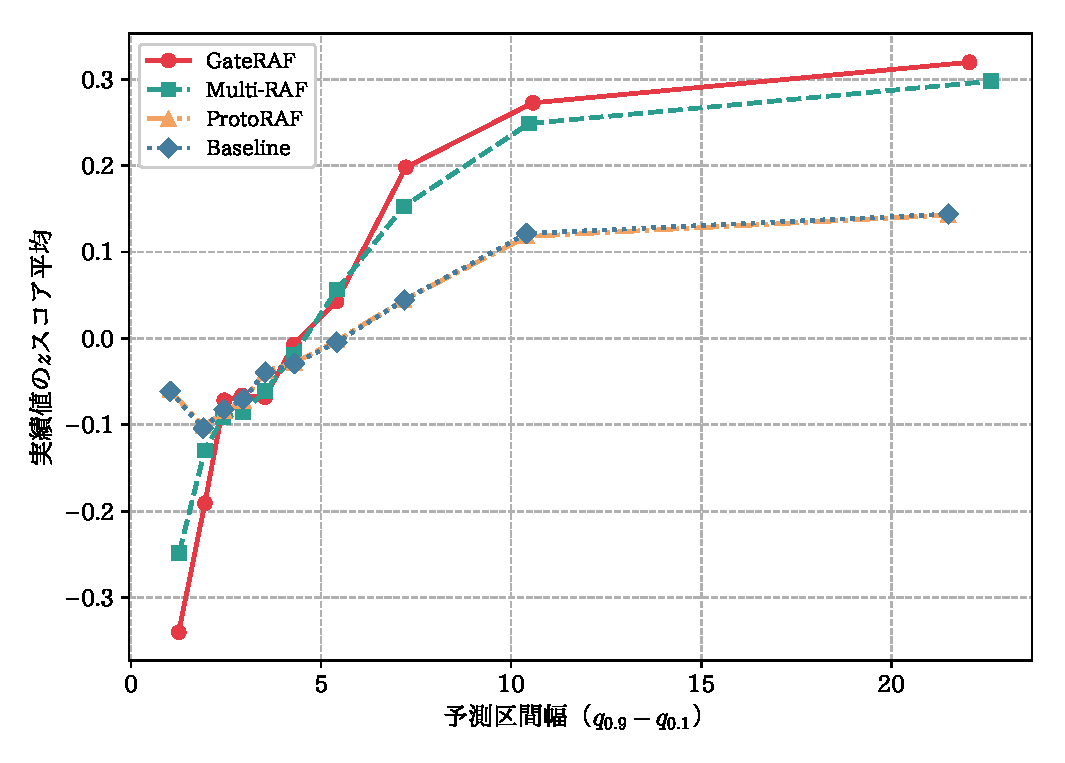
\includegraphics[width=\linewidth]{figure/interval_calibration.eps}
        \caption{予測区間の幅ごとの実績$z$スコア平均}
        \label{Fig:interval_calibration}
    \end{figure}


\subsubsection{実験5：代表系列の事例分析}
現れ方の異なる代表的な2系列について，各手法の$\tau=0.5$の予測を実績と重ねて比較した結果を図~\ref{fig:book_examples}に示す．このうち，図~\ref{fig:book_bocchi}に示す書籍Aは，高い需要が時間とともに減衰する系列である．GateRAFは実績の減衰にほぼ沿って予測を下げるのに対し，ProtoRAF・Baselineは需要が下がった後も高い予測を維持している．
これは，ProtoRAFが連結系列全体で標準化するため予測のスケールが過大なまま保たれるためであると考えられ，標準化を局所化するGateRAFではこの高止まりが避けられている．

図~\ref{fig:book_crossword}に示す書籍Bは，平常はほぼゼロの需要が突発的に急増する系列である．
GateRAFとMulti-RAFは販売冊数の急増に合わせて予測値も上昇しているのに対し，
ProtoRAF, Baselineはほぼゼロのまま反応せず，加法モデルのProphetも構造上この急増を表現できていない．
GateRAF, Multi-RAF共に同様の傾向が見られることから，スパイクの捕捉は主にマルチストリームエンコードの働きによると考えられる．
%%% [REV-A7] スパイク時点に限定した評価との対応づけ（査読者#A コメント7）ここから
\revA{ただし書籍Bでは，予測の上昇は実績の急増に比べて小さく，スパイクの水準までは再現できていない．なお，スパイクの時点だけに限った評価は表~\ref{tab:mae_rmse_vs_zscore}の$z$スコアが$2$以上の区分に，スパイクの位置のずれの評価は表~\ref{tab:temporal_proximity}に示している．また，スパイクの高さの再現と上側分位点による被覆については5.4.2項で述べた通りである．}
%%% [REV-A7] ここまで

これら2例は，いずれもマルチストリームエンコードの効果，すなわち標準化の局所化による過大予測の抑制と，参照の個別取り込みによる他系列スパイクの捕捉を示している．ゲート機構の寄与はこれとは異なり，実験1・2の平常時（下側分位点・静穏域）の精度向上と，実験3のスパイク近傍への時間的な絞り込みに現れる．
        \begin{figure*}[tb]
            \centering
            \begin{subfigure}[t]{0.8\textwidth}
                \centering
                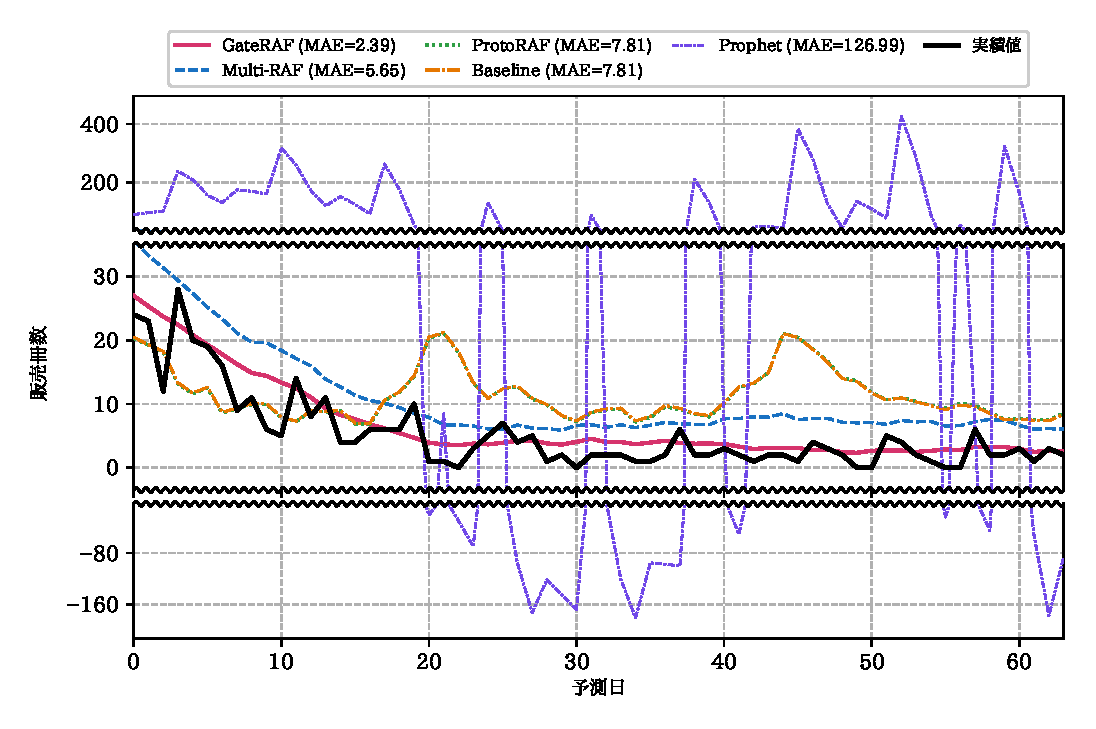
\includegraphics[width=\linewidth]{figure/figure_book/bocchi/figure_book_bocchi_prophet.eps}
                \caption{書籍A}
                \label{fig:book_bocchi}
            \end{subfigure}
            \begin{subfigure}[t]{0.8\textwidth}
                \centering
                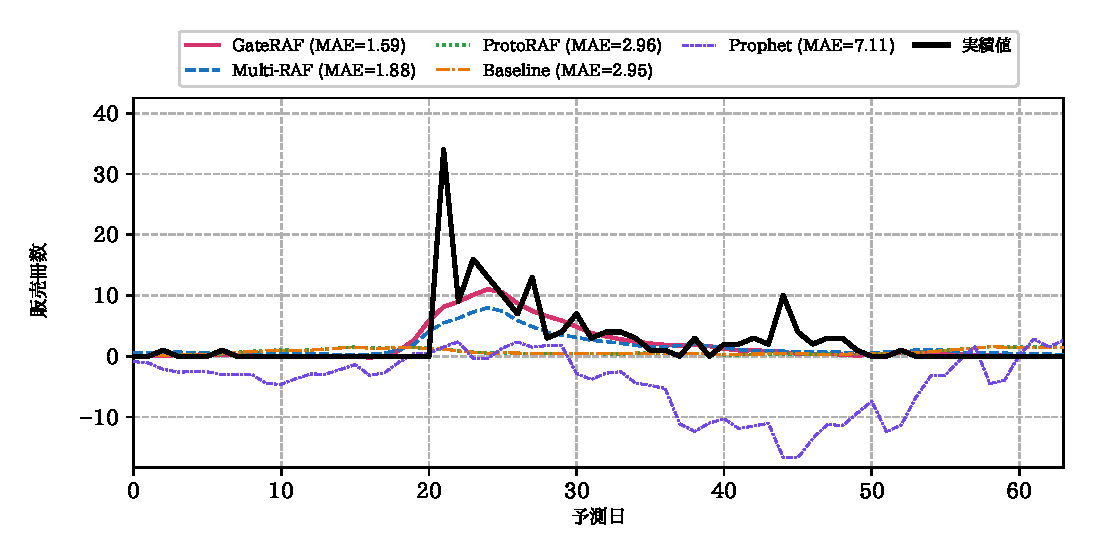
\includegraphics[width=\linewidth]{figure/figure_book/crossword/figure_book_crossword_prophet.eps}
                \caption{書籍B}
                \label{fig:book_crossword}
            \end{subfigure}
            \caption{各系列における予測と実績の比較}
            \label{fig:book_examples}
        \end{figure*}

%%%%%%%%%%%%%%%%%%%%%%%%%%%%%%%%%%%%%%%%%%%%%%%%%%%%%%%%%%%%%%%%%%%%%%%%%%%%%%%
\section{返本と機会損失の観点からの評価}
%%%%%%%%%%%%%%%%%%%%%%%%%%%%%%%%%%%%%%%%%%%%%%%%%%%%%%%%%%%%%%%%%%%%%%%%%%%%%%%
以下では，予測誤差が出版流通にもたらす損失を，返本と販売機会の損失という実務的な観点から評価する．需要を上回る入荷は売れ残りとなって返本を生み，過剰な返本は出版流通全体の課題となっている．一方で，需要のスパイクに見合う入荷ができなければ機会損失が生じる．
そこで，各手法が予測した販売冊数をそのまま入荷量とみなし，提案手法GateRAFが返本と販売機会の損失をどの程度抑えられるかを，他手法との比較により見積もる．
MAEやRMSEといった精度指標は，予測の良し悪しを数値としては示すものの，それが出版流通の現場でどれだけの負担や損失につながるのかを直接には表さない．そこで以下では，予測精度の違いを返本と機会損失という実務的な指標へと結び付けることで，提案手法が出版流通の効率化にもたらす意義を明らかにする．なお本評価は，発注リードタイムや在庫の繰り越しといった実際の流通過程を含まない簡易的なシミュレーションであり，損失量そのものではなく手法間の相対的な差を把握することを目的とする．比較対象には，基盤モデルそのものであるBaselineに加え，古典的な予測手法であるSARIMA~\cite{Box.1970}とProphet~\cite{Taylor.2018}を用いる．

評価指標は，過剰入荷$O$，返本率$R$，機会損失$U$の3つである．評価対象とする全書名について，評価期間である$F=64$日にわたり，時点$t$の実際の販売冊数を$y_t$，予測した販売冊数の中央値（$\tau=0.5$）を$\hat{y}_t$とし，$\hat{y}_t$をその時点の入荷量とみなす．入荷量が実際の販売を上回った分を売れ残りとして合計したものが過剰入荷$O$であり，これがそのまま返本となる．
一方，入荷量が実際の販売に届かなかった分を合計したものが機会損失$U$である．返本率$R$は，実際の総販売冊数$S=\sum_t y_t$と過剰入荷の和に対し，過剰入荷が占める割合とする．以上をまとめると，3つの指標は次のように表される．
    \begin{align}
        O &= \sum_t \max(\hat{y}_t - y_t,\, 0) \\
        U &= \sum_t \max(y_t - \hat{y}_t,\, 0) \\
        R &= \frac{O}{S + O}
    \end{align}
返本率$R$が高いほど返品にともなう物流の負担が大きく，機会損失$U$が大きいほど，入荷が需要に満たず，本来得られたはずの販売機会を多く逸失していることを意味する．
%%% [REV-B7] 入荷量に用いる分位点の感度分析（査読者#B コメント7）ここから
\revBblock{
入荷量に中央値（$\tau=0.5$）を用いたのは，返本と機会損失のどちらにも重みを置かない中立的な基準だからである．どちらの損失をどれだけ重くみるかは実務の費用構造によって異なるため，本研究では特定の費用構造を仮定せず，入荷を需要の中心に合わせる場合を基準とした．

$\tau$の選び方による違いを表~\ref{tab:quantile_sensitivity}に示す．$\tau=0.1$では入荷を絞るため過剰入荷はGateRAFで$4{,}073$冊まで減るが，機会損失は$265{,}006$冊と$\tau=0.5$の約$1.6$倍になる．逆に$\tau=0.9$では機会損失が$74{,}763$冊まで下がる一方，過剰入荷は$296{,}482$冊に達する．

手法間の関係は$\tau$によらず保たれる．いずれの$\tau$でもGateRAFの過剰入荷は比較手法の中で最小であり，Baselineに対しては過剰入荷と機会損失の双方を同時に下回る．すなわち以下の結果は，入荷量にどの分位点を用いるかに依存しない．
}
%%% [REV-B7] ここまで

\begin{table*}[t]
    \revBcolor
    \caption{入荷量に用いる分位点$\tau$を変えた場合の過剰入荷および機会損失［冊］}
    \label{tab:quantile_sensitivity}
    \centering
    \setlength{\tabcolsep}{6pt}%
    \begin{tabular}{lrrrrrr}
        \hline
        & \multicolumn{2}{c}{$\tau=0.1$} & \multicolumn{2}{c}{$\tau=0.5$} & \multicolumn{2}{c}{$\tau=0.9$} \\
        \cline{2-3} \cline{4-5} \cline{6-7}
        \multicolumn{1}{c}{モデル} & \multicolumn{1}{c}{過剰入荷} & \multicolumn{1}{c}{機会損失} & \multicolumn{1}{c}{過剰入荷} & \multicolumn{1}{c}{機会損失} & \multicolumn{1}{c}{過剰入荷} & \multicolumn{1}{c}{機会損失} \\
        \hline\hline
        \textbf{GateRAF} & \textbf{4{,}073} & \textbf{265{,}006} & \textbf{41{,}182} & 162{,}098 & \textbf{296{,}482} & 74{,}763 \\
        \textbf{Baseline} & 4{,}271 & 266{,}008 & 57{,}383 & 168{,}171 & 428{,}864 & 78{,}453 \\
        \textbf{SARIMA} & 4{,}315 & 642{,}766 & 124{,}588 & \textbf{150{,}440} & 657{,}493 & \textbf{70{,}746} \\
        \textbf{Prophet} & 219{,}753 & 917{,}871 & 331{,}923 & 317{,}997 & 910{,}309 & 185{,}874 \\
        \hline
    \end{tabular}
\end{table*}

以下では$\tau=0.5$を入荷量とみなした場合について詳しくみる．返本率と，本体価格により金額換算した損失額を表~\ref{tab:return_loss}に示す．
    \begin{table}[t]
        \caption{予測値\revB{（$\tau=0.5$）}を入荷量とみなした場合の返本率\revAcolor と損失額（本体価格による換算）}
        \label{tab:return_loss}
        \centering
        \setlength{\tabcolsep}{6pt}%
        \begin{tabular}{lrrr}
            \hline
            & & \multicolumn{2}{c}{\revAcolor 金額［万円］} \\
            \cline{3-4}
            \multicolumn{1}{c}{モデル} & \multicolumn{1}{c}{返本率} & \multicolumn{1}{c}{\revAcolor 過剰入荷} & \multicolumn{1}{c}{\revAcolor 機会損失} \\
            \hline\hline
            \textbf{GateRAF} & \textbf{12.33\%} & \revAcolor\textbf{3{,}173} & \revAcolor 12{,}052 \\
            \textbf{Baseline} & 16.39\% & \revAcolor 4{,}401 & \revAcolor 12{,}384 \\
            \textbf{SARIMA} & 29.85\% & \revAcolor 9{,}361 & \revAcolor\textbf{11{,}239} \\
            \textbf{Prophet} & 53.13\% & \revAcolor 23{,}170 & \revAcolor 23{,}607 \\
            \hline
        \end{tabular}
    \end{table}

まず，参照を用いないBaselineとの比較から，提案手法の効果を確認する．GateRAFはBaselineに対し，返本率を$16.4\%$から$12.3\%$へ下げ，機会損失も$168{,}171$から$162{,}098$へと同時に減らした．予測精度の改善が，売れ残りと売り逃しの双方の削減として現れている．次に古典的手法と比較すると，GateRAFの返本率はSARIMAの$29.9\%$，Prophetの$53.1\%$を大きく下回る．過剰入荷の冊数で比較しても，GateRAFはSARIMAの約3分の1，Prophetの約8分の1にとどまる．一方で機会損失はSARIMAが最小であり，GateRAFはこれを約$8\%$上回る$162{,}098$冊であった．

返本と機会損失は，本来両立の難しい指標である．売り逃しを減らそうとして入荷を増やせば，売れ残りが増えて返本が増大するためである．SARIMAは入荷量を多めに見積もることで機会損失を最小に抑えるが，過剰入荷はGateRAFの約3倍に達し，返本率もGateRAFの2倍を超える．これに対しGateRAFは，機会損失の増加を最小手法であるSARIMAに対して約$8\%$にとどめつつ，返本を大幅に抑えている．返本の抑制が出版流通全体の課題であることを踏まえると，GateRAFは販売機会の損失を低い水準に保ったまま返本を抑えており，実務上望ましい特性を備えていることが示唆された．
%%% [REV-A8] 金額換算による実務的インパクトの提示（査読者#A コメント8）ここから
\revA{これらを本体価格で金額に換算すると，GateRAFの過剰入荷は$3{,}173$万円，機会損失は$1$億$2{,}052$万円となる．Baselineと比べると返本が$1{,}228$万円，機会損失が$332$万円減り，提案手法を用いることで約$1{,}560$万円の損失を抑えられることが示唆される．評価対象は$1{,}157$書名の$64$日分（本体価格ベースの売上$2$億$1{,}369$万円）であり，返本の抑制が金額でも相応の規模になることがわかる．}

\revA{また，返本は書店から取次・出版社への返品であり，往復の輸送と在庫の再処理を伴う．GateRAFはBaselineに対し返本を$16{,}201$冊減らしており，その分の物流コストが低減可能となる．加えて，委託販売制度のもとでは売れ残りの在庫リスクを出版社が負うため，過剰入荷の抑制はそのリスクの軽減を可能とする．GateRAFは機会損失も同時に$6{,}073$冊減らしており，欠品を増やさずに実現可能であることからもその有効性を示すことができた．}
%%% [REV-A8] ここまで


%%%%%%%%%%%%%%%%%%%%%%%%%%%%%%%%%%%%%%%%%%%%%%%%%%%%%%%%%%%%%%%%%%%%%%%%%%%%%%%
\section{おわりに}
%%%%%%%%%%%%%%%%%%%%%%%%%%%%%%%%%%%%%%%%%%%%%%%%%%%%%%%%%%%%%%%%%%%%%%%%%%%%%%%
本研究では，平常時とスパイクが混在する書籍の需要予測を目的に，GateRAFを提案した．GateRAFは，従来のRAFがもつ接合部の不連続性をマルチストリームエンコードによって構造的に取り除き，無関係な参照の混入をゲート機構によって動的に抑制する．実験の結果，GateRAFは全体の予測精度でProtoRAFとBaselineを上回り，2つの機構が予測の異なる側面を改善することを確認した．

今後の課題として，形状以外の観点も取り入れた類似尺度，参照を組み合わせたゲート機構の検討などが挙げられる．

%% 謝辞
%\shaji
%貴重なデータをご提供いただいた企業様を始め，データ解析コンペティション関係者の皆様にお礼申し上げます．　


%%%%%%%% 参考文献 %%%%%%%%%%%%%%%%%%%%%%%%%%%%%%%%%%%%%%%%%%%%%%%%%%%%%%%%%%%%%%

\begin{thebibliography}{99}

\bibitem[日本書籍出版協会(2001)]{JBPA.2001}
日本書籍出版協会,
「再販制度」,
\url{https://www.jbpa.or.jp/resale/}, 2001（2026年6月26日閲覧）.

\bibitem[全国出版協会・出版科学研究所(2024)]{Shuppan.2024}
全国出版協会・出版科学研究所,
『出版指標年報 2024年版』,
全国出版協会, 2024.

\bibitem[Lewis~et~al.(2020)]{Lewis.2020}
P.~Lewis, E.~Perez, A.~Piktus, F.~Petroni, V.~Karpukhin, N.~Goyal, H.~K\"{u}ttler, M.~Lewis, W.-T.~Yih, T.~Rockt\"{a}schel, S.~Riedel and D.~Kiela,
``Retrieval-Augmented Generation for Knowledge-Intensive {NLP} Tasks,''
in \textit{Advances in Neural Information Processing Systems}, vol.~33, pp.~9459--9474, 2020.

\bibitem[Tire~et~al.(2024)]{Tire.2024}
K.~Tire, E.~O.~Taga, M.~E.~Ildiz and S.~Oymak,
``Retrieval Augmented Time Series Forecasting,''
arXiv:2411.08249, 2024.

\bibitem[Nie~et~al.(2023)]{Nie.2023}
Y.~Nie, N.~H.~Nguyen, P.~Sinthong and J.~Kalagnanam,
``A Time Series is Worth 64 Words: Long-term Forecasting with Transformers,''
in \textit{Proceedings of the International Conference on Learning Representations}, 2023.

\bibitem[Salinas~et~al.(2020)]{Salinas.2020}
D.~Salinas, V.~Flunkert, J.~Gasthaus and T.~Januschowski,
``{DeepAR}: Probabilistic Forecasting with Autoregressive Recurrent Networks,''
\textit{International Journal of Forecasting}, vol.~36, no.~3, pp.~1181--1191, 2020.

\bibitem[Lim~et~al.(2021)]{Lim.2021}
B.~Lim, S.~\"{O}.~Ar{\i}k, N.~Loeff and T.~Pfister,
``Temporal Fusion Transformers for Interpretable Multi-Horizon Time Series Forecasting,''
\textit{International Journal of Forecasting}, vol.~37, no.~4, pp.~1748--1764, 2021.

\bibitem[Ansari~et~al.(2024)]{Ansari.2024}
A.~F.~Ansari, L.~Stella, C.~Turkmen, X.~Zhang, P.~Mercado, H.~Shen, O.~Shchur,
S.~S.~Rangapuram, S.~P.~Arango, S.~Kapoor, J.~Zschiegner, D.~C.~Maddix,
H.~Wang, M.~W.~Mahoney, K.~Torkkola, A.~G.~Wilson, M.~Bohlke-Schneider and Y.~Wang,
``Chronos: Learning the Language of Time Series,''
arXiv:2403.07815, 2024.


\bibitem[Croston(1972)]{Croston.1972}
J.~D.~Croston,
``Forecasting and Stock Control for Intermittent Demands,''
\textit{Operational Research Quarterly}, vol.~23, no.~3, pp.~289--303, 1972.

\bibitem[Ning~et~al.(2025)]{Ning.2025}
K.~Ning, Z.~Pan, Y.~Liu, Y.~Jiang, J.~Y.~Zhang, K.~Rasul, A.~Schneider, L.~Ma, Y.~Nevmyvaka and D.~Song,
``TS-RAG: Retrieval-Augmented Generation based Time Series Foundation Models are Stronger Zero-Shot Forecaster,''
arXiv:2503.07649, 2025.

\bibitem[Zhang~et~al.(2024)]{Zhang.2024}
H.~Zhang, C.~Xu, Y.-F.~Zhang, Z.~Zhang, L.~Wang, J.~Bian and T.~Tan,
``{TimeRAF}: Retrieval-Augmented Foundation Model for Zero-Shot Time Series Forecasting,''
arXiv:2412.20810, 2024.

%%% [REV-A1] Faissの文献を復活（査読者#A コメント1）ここから
%%% [REV-A1] 類似尺度の頑健性に関する文献の追加（査読者#A コメント1）ここから
\bibitem[Lee~et~al.(2026)]{Lee.2026}
S.~Lee, J.~Lee, J.~Seo, S.~Yoo, M.~Kim, T.~Y.~Lim, D.~Kang, H.~Choi, S.~Lee and W.~Ahn,
``Cross-RAG: Zero-Shot Retrieval-Augmented Time Series Forecasting via Cross-Attention,''
arXiv:2603.14709, 2026.
%%% [REV-A1] ここまで

\bibitem[Johnson~et~al.(2019)]{Johnson.2019}
J.~Johnson, M.~Douze and H.~J\'{e}gou,
``Billion-Scale Similarity Search with {GPU}s,''
\textit{IEEE Transactions on Big Data}, vol.~7, no.~3, pp.~535--547, 2019.
%%% [REV-A1] ここまで

\bibitem[Kim~et~al.(2022)]{Kim.2022}
T.~Kim, J.~Kim, Y.~Tae, C.~Park, J.-H.~Choi and J.~Choo,
``Reversible Instance Normalization for Accurate Time-Series Forecasting against Distribution Shift,''
in \textit{Proceedings of the International Conference on Learning Representations}, 2022.

\bibitem[Liu~et~al.(2024)]{Liu.2024}
S.-Y.~Liu, C.-Y.~Wang, H.~Yin, P.~Molchanov, Y.-C.~F.~Wang, K.-T.~Cheng and M.-H.~Chen,
``{DoRA}: Weight-Decomposed Low-Rank Adaptation,''
in \textit{Proceedings of the International Conference on Machine Learning}, 2024.

\bibitem[Taylor~\&~Letham(2018)]{Taylor.2018}
S.~J.~Taylor and B.~Letham,
``Forecasting at Scale,''
\textit{The American Statistician}, vol.~72, no.~1, pp.~37--45, 2018.

\bibitem[Koenker~\&~Bassett(1978)]{Koenker.1978}
R.~Koenker and G.~W.~Bassett,
``Regression Quantiles,''
\textit{Econometrica}, vol.~46, no.~1, pp.~33--50, 1978.

\bibitem[Box~\&~Jenkins(1970)]{Box.1970}
G.~E.~P.~Box and G.~M.~Jenkins,
\textit{Time Series Analysis: Forecasting and Control},
Holden-Day, 1970.

\end{thebibliography}

\end{document}
